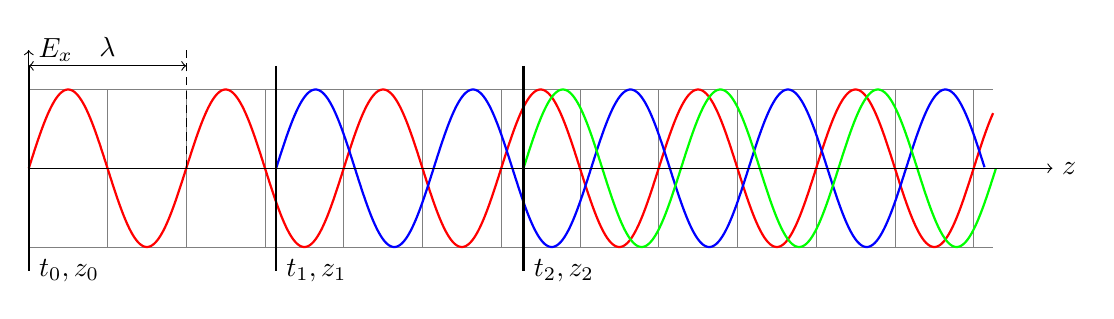
\begin{tikzpicture}

  \draw [help lines] (0,-1) grid (12.25,1);

  \draw[thick, red] plot[domain=0:12.25*pi, samples=1000]  (\x/pi,{sin(\x r)});


  \draw[densely dashed]   (0,0) -- + (0,1.5)      (2,0) -- + (0,1.5);
  \draw[<->]      (0,1.3) -- node[above] {$\lambda$} + (2,0);

  \draw[thick, blue] plot[domain=0:9*pi, samples=1000]  (\x/pi + 1*pi,{sin(\x r)});

  \draw[thick, green] plot[domain=0:6*pi, samples=1000]  (\x/pi + 2*pi,{sin(\x r)});
  \draw[thick, black] (2*pi,+1.3) --  (2*pi,-1.3) node[right] {$t_2, z_2$} ;
  \draw[thick, black] (pi,+1.3) --  (pi,-1.3) node[right] {$t_1, z_1$} ;
  \draw[thick, black] (0,+1.3) -- (0,-1.3) node[right] {$t_0, z_0$};
  \draw[->]   (0,0) -- ++ (13,0) node[right] {$z$};
  \draw[->]   (0,0) -- ++ (0,1.5) node[right] {$E_x$};
\end{tikzpicture}